\documentclass[12pt, a4paper]{article}
% Packages: 
\usepackage[utf8]{inputenc}
\usepackage[T1]{fontenc}
\usepackage[polish]{babel}
\usepackage[utf8]{inputenc}
\usepackage{lmodern}
\usepackage{graphicx}
\usepackage{indentfirst}
\usepackage{fancyhdr}
%------------------------------------
% Style config etc.:
\selectlanguage{polish}
\brokenpenalty=1000
\clubpenalty=1000
\widowpenalty=1000    
\pagestyle{fancy}
\fancyhead{}
\fancyfoot{}
\rfoot{\thepage}
\lfoot{}
\lhead{}
\rhead{}
\renewcommand{\headrulewidth}{1pt}
\renewcommand{\footrulewidth}{1pt}
%--------------------
\title{Tworzenie obrazu kontenera dla prostej aplikacji}
\author{Marian Dorosz}
\date{}
\begin{document}

\maketitle
\thispagestyle{empty}
\newpage
\tableofcontents
\newpage
\listoffigures
\newpage
\section{Problem do rozwiązania}
    Należy zbudować \textbf{obraz kontenera} aplikacji napisanej przy pomocy \textbf{node.js}. Po zbudowaniu obrazu utworzyć plik typu \textbf{docker-compose}, którego zadaniem będzie uruchomienie kontenera z bazą mongoDB w wersji 3 oraz kontenera z aplikacją, który miał być utworzony. Po uruchomieniu pliku docker-compose sprawdzić poleceniem \textbf{curl} poprawność działania systemu. Po poprawnym zainicjowaniu kontenerów wynikiem polecenia \textbf{curl} powinien być napis \textbf{"Hello World!"}.
\section{Rozwiązanie problemu}
    \subsection{Kod aplikacji}
        \begin{figure}[!h]
            \centering
            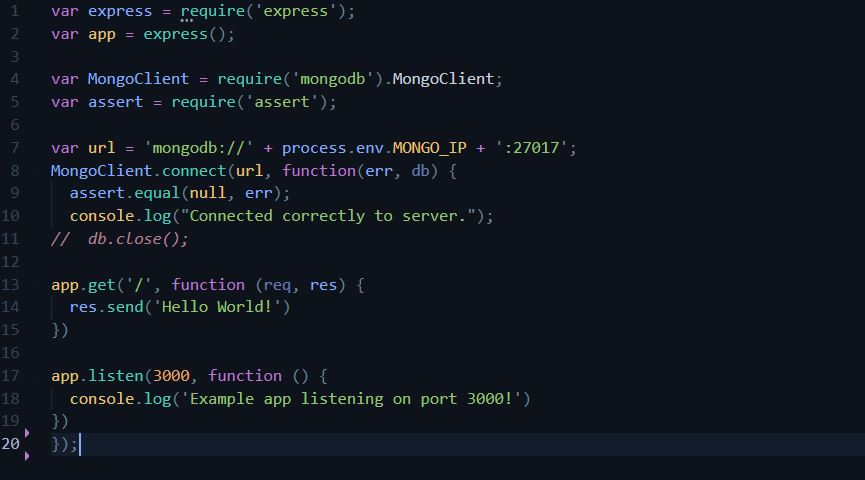
\includegraphics[width=\textwidth]{aplikacja.JPG}
            \caption{Kod aplikacji node.js}
            \label{fig:aplikacja}
        \end{figure}
    \newpage
    \subsection{Plik Dockerfile}
        \begin{figure}[!h]
            \centering
            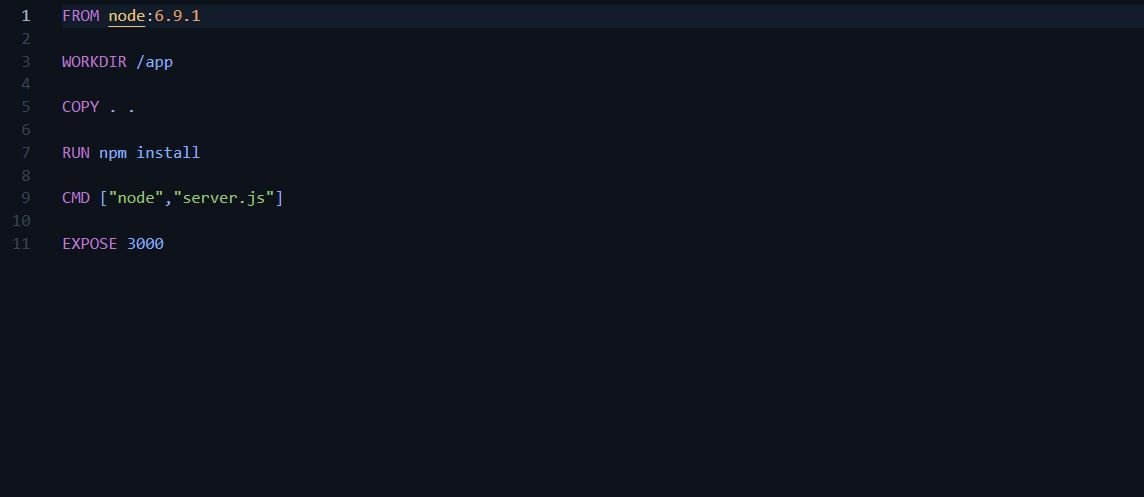
\includegraphics[width = \textwidth]{docker-file.JPG}
            \caption{Kod znajdujący się w pliku Dockerfile}
            \label{fig:dockerfile}
        \end{figure}
        \subsubsection{FROM} 
            Instrukcja \textbf{From} oznacza na podstawie jakiego obrazu będzie budowany obraz kontenera. Jak widać na załączonym obrazku tworzony obraz będzie posiadać funkcjonalności kontenera node:6.9.1.
        \subsubsection{WORKDIR} 
            Polecenie \textbf{WORKDIR} ustawia ścieżkę, w której będzie wykonywana każda komenda (np.: RUN, CMD itp.). Jeżeli dana ścieżka nie istnieje, to zostanie utworzona. Warto dodać, że wszystko będzie odbywać się wewnątrz kontenera. W tym przypadku będzie to folder \textbf{/app}.
        \subsubsection{COPY} 
            Polecenie to kopiuje pliki z lokalnej maszyny do pamięci kontenera. W powyższym przypadku wszystkie pliki, które znajdują w folderze wraz z plikiem \textbf{Dockerfile} zostaną przekopiowane do folderu \textbf{/app}.
        \subsubsection{RUN}
            Polecenie \textbf{RUN} uruchamia polecenia podane jako argumenty w trakcie budowania kontenera. Wykonają się one jednorazowo. W przypadku tego kontenera zostało uruchomione polecenie \textbf{npm install}, które zainstaluje wszystkie zależności potrzebne do uruchomienia aplikacji.
        \subsubsection{CMD}
            Polecenie \textbf{CMD} przyjmuje jako argumenty komendy, które mają zostać wykonane przy każdym uruchomieniu kontenera. W tym wypadku będzie to uruchomienie skryptu o nazwie \textbf{server.js} przez aplikację \textbf{node}.
        \subsubsection{EXPOSE}
            \textbf{EXPOSE} to informacja dla osoby, która będzie używać kontenera. Przyjmuje ona jako argument numer portu oraz rodzaj protokołu. Ma ona sygnalizować jakie porty mają zostać wykorzystane w trakcie używania komendy \textbf{docker run}.
    \subsection{Wynik polecenia docker build}
        \begin{figure}[!h]
            \centering
            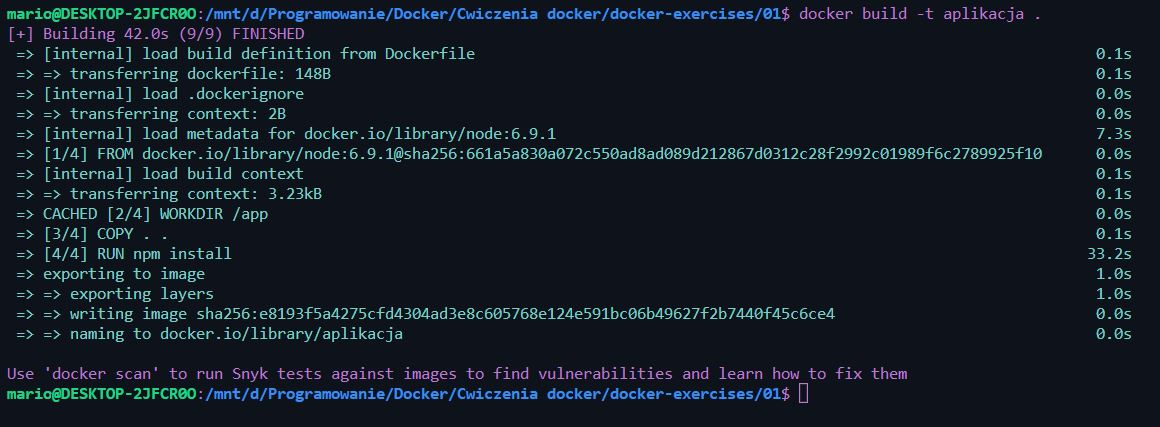
\includegraphics[width=\textwidth]{docker-build.JPG}
            \caption{Wynik polecenia docker build}
            \label{fig:my_label}
        \end{figure}
        Polecenie docker build konstruuje obraz kontenera wykorzystując polecenia znajdujące się w pliku \textbf{Dockerfile}. Jak widać obraz został poprawnie utworzony, gdyż nie zostały zakomunikowane żadne błędy.
\newpage
    \subsection{Plik docker compose oraz wynik jego uruchomienia}
        \begin{figure}[!h]
            \centering
            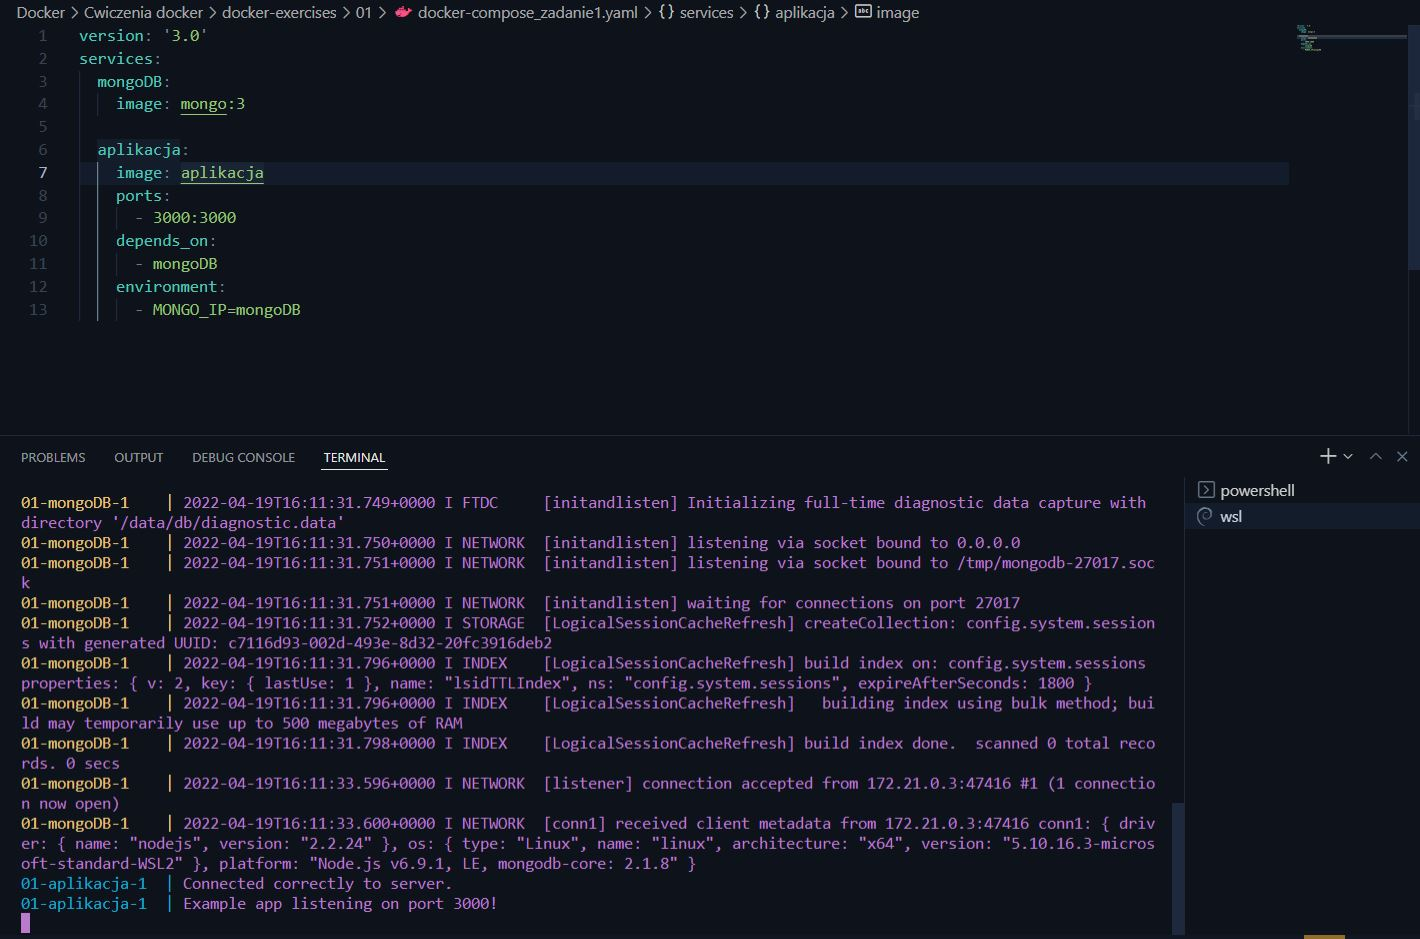
\includegraphics[width=\textwidth]{docker-compose.JPG}
            \caption{Zawartość pliku docker compose oraz wynik egzekucji}
            \label{fig:dockercompose}
        \end{figure}
        Jak widać na powyższym rysunku udało się uruchomić obie usługi, o czym świadczy komunikat \textbf{Connected correctly to server}.
    \subsection{Wynik polecenia curl.}
        \begin{figure}[!h]
            \centering
            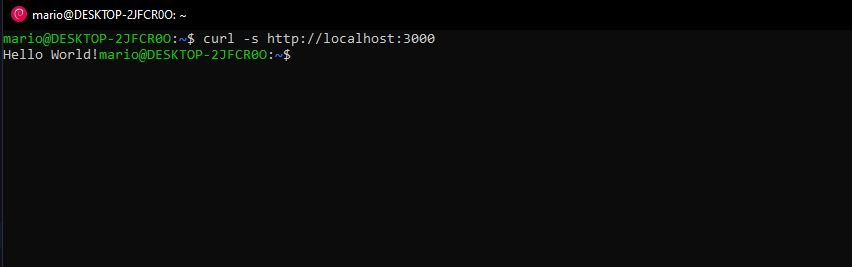
\includegraphics[width=\textwidth]{curl.JPG}
            \caption{Wynik polecenia curl}
            \label{fig:curl}
        \end{figure}
        Jak widać wszystko zostało skonfigurowane poprawnie, ponieważ polecenie curl zwróciło napis \textbf{Hello World!}
    \section{Źródła}
    Autor aplikacji nodejs: github.com/Vizuri
\end{document}
\documentclass[12pt, a4paper]{article}
% Packages: 
\usepackage[utf8]{inputenc}
\usepackage[T1]{fontenc}
\usepackage[polish]{babel}
\usepackage[utf8]{inputenc}
\usepackage{lmodern}
\usepackage{graphicx}
\usepackage{indentfirst}
\usepackage{fancyhdr}
%------------------------------------
% Style config etc.:
\selectlanguage{polish}
\brokenpenalty=1000
\clubpenalty=1000
\widowpenalty=1000    
\pagestyle{fancy}
\fancyhead{}
\fancyfoot{}
\rfoot{\thepage}
\lfoot{}
\lhead{}
\rhead{}
\renewcommand{\headrulewidth}{1pt}
\renewcommand{\footrulewidth}{1pt}
%--------------------
\title{Tworzenie obrazu kontenera dla prostej aplikacji}
\author{Marian Dorosz}
\date{}
\begin{document}

\maketitle
\thispagestyle{empty}
\newpage
\tableofcontents
\newpage
\listoffigures
\newpage
\section{Problem do rozwiązania}
    Należy zbudować \textbf{obraz kontenera} aplikacji napisanej przy pomocy \textbf{node.js}. Po zbudowaniu obrazu utworzyć plik typu \textbf{docker-compose}, którego zadaniem będzie uruchomienie kontenera z bazą mongoDB w wersji 3 oraz kontenera z aplikacją, który miał być utworzony. Po uruchomieniu pliku docker-compose sprawdzić poleceniem \textbf{curl} poprawność działania systemu. Po poprawnym zainicjowaniu kontenerów wynikiem polecenia \textbf{curl} powinien być napis \textbf{"Hello World!"}.
\section{Rozwiązanie problemu}
    \subsection{Kod aplikacji}
        \begin{figure}[!h]
            \centering
            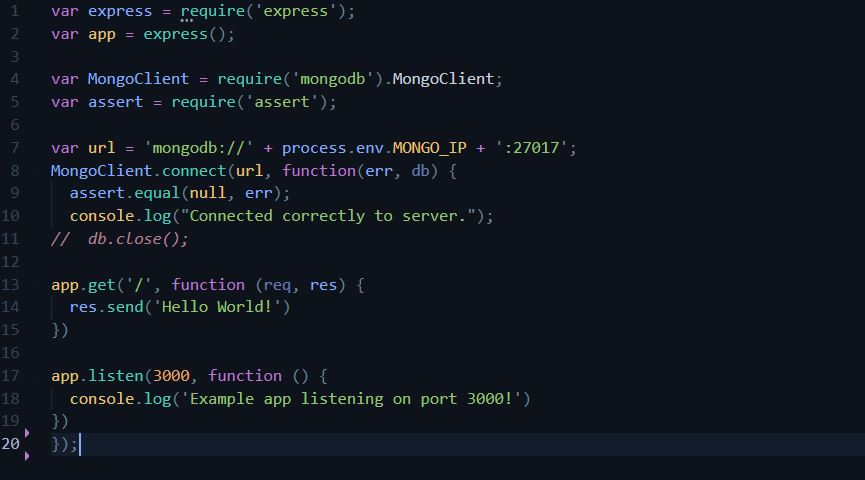
\includegraphics[width=\textwidth]{aplikacja.JPG}
            \caption{Kod aplikacji node.js}
            \label{fig:aplikacja}
        \end{figure}
    \newpage
    \subsection{Plik Dockerfile}
        \begin{figure}[!h]
            \centering
            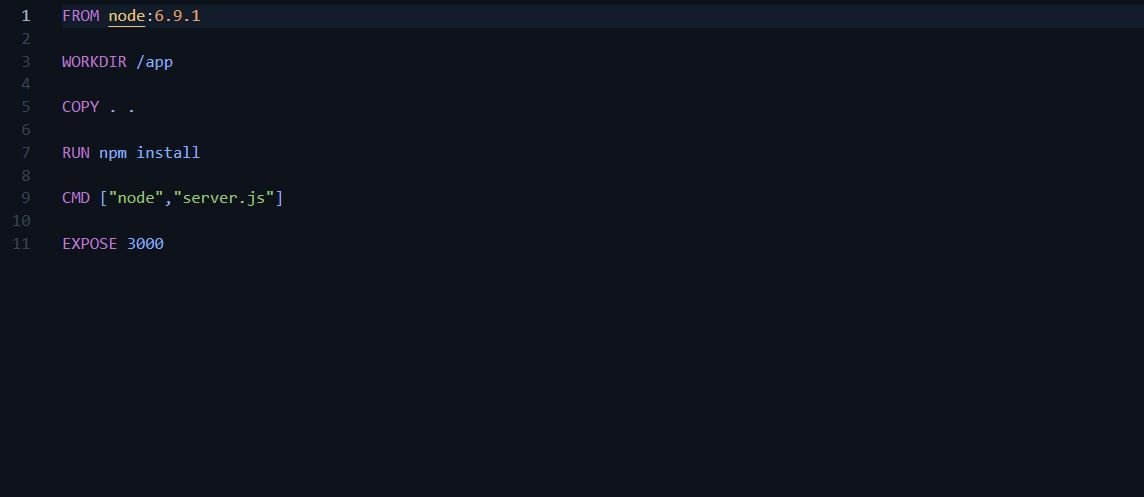
\includegraphics[width = \textwidth]{docker-file.JPG}
            \caption{Kod znajdujący się w pliku Dockerfile}
            \label{fig:dockerfile}
        \end{figure}
        \subsubsection{FROM} 
            Instrukcja \textbf{From} oznacza na podstawie jakiego obrazu będzie budowany obraz kontenera. Jak widać na załączonym obrazku tworzony obraz będzie posiadać funkcjonalności kontenera node:6.9.1.
        \subsubsection{WORKDIR} 
            Polecenie \textbf{WORKDIR} ustawia ścieżkę, w której będzie wykonywana każda komenda (np.: RUN, CMD itp.). Jeżeli dana ścieżka nie istnieje, to zostanie utworzona. Warto dodać, że wszystko będzie odbywać się wewnątrz kontenera. W tym przypadku będzie to folder \textbf{/app}.
        \subsubsection{COPY} 
            Polecenie to kopiuje pliki z lokalnej maszyny do pamięci kontenera. W powyższym przypadku wszystkie pliki, które znajdują w folderze wraz z plikiem \textbf{Dockerfile} zostaną przekopiowane do folderu \textbf{/app}.
        \subsubsection{RUN}
            Polecenie \textbf{RUN} uruchamia polecenia podane jako argumenty w trakcie budowania kontenera. Wykonają się one jednorazowo. W przypadku tego kontenera zostało uruchomione polecenie \textbf{npm install}, które zainstaluje wszystkie zależności potrzebne do uruchomienia aplikacji.
        \subsubsection{CMD}
            Polecenie \textbf{CMD} przyjmuje jako argumenty komendy, które mają zostać wykonane przy każdym uruchomieniu kontenera. W tym wypadku będzie to uruchomienie skryptu o nazwie \textbf{server.js} przez aplikację \textbf{node}.
        \subsubsection{EXPOSE}
            \textbf{EXPOSE} to informacja dla osoby, która będzie używać kontenera. Przyjmuje ona jako argument numer portu oraz rodzaj protokołu. Ma ona sygnalizować jakie porty mają zostać wykorzystane w trakcie używania komendy \textbf{docker run}.
    \subsection{Wynik polecenia docker build}
        \begin{figure}[!h]
            \centering
            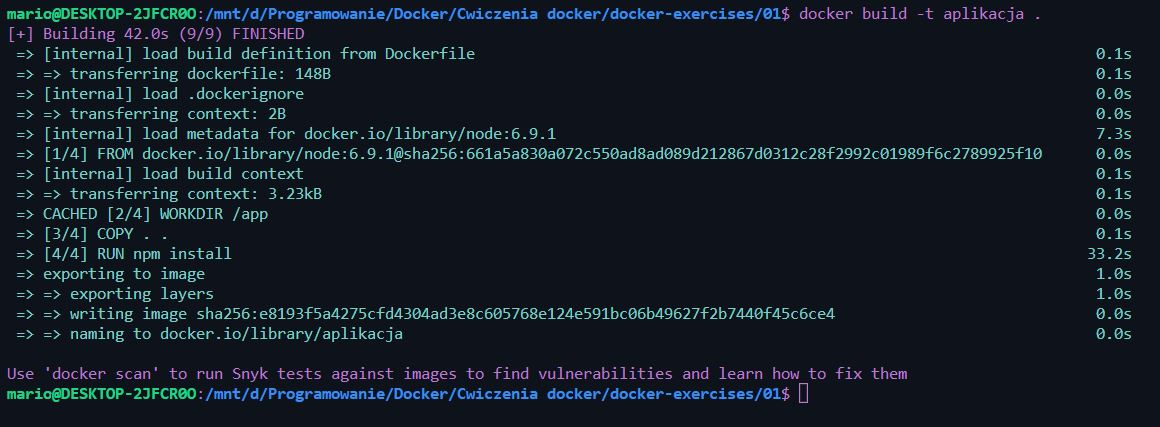
\includegraphics[width=\textwidth]{docker-build.JPG}
            \caption{Wynik polecenia docker build}
            \label{fig:my_label}
        \end{figure}
        Polecenie docker build konstruuje obraz kontenera wykorzystując polecenia znajdujące się w pliku \textbf{Dockerfile}. Jak widać obraz został poprawnie utworzony, gdyż nie zostały zakomunikowane żadne błędy.
\newpage
    \subsection{Plik docker compose oraz wynik jego uruchomienia}
        \begin{figure}[!h]
            \centering
            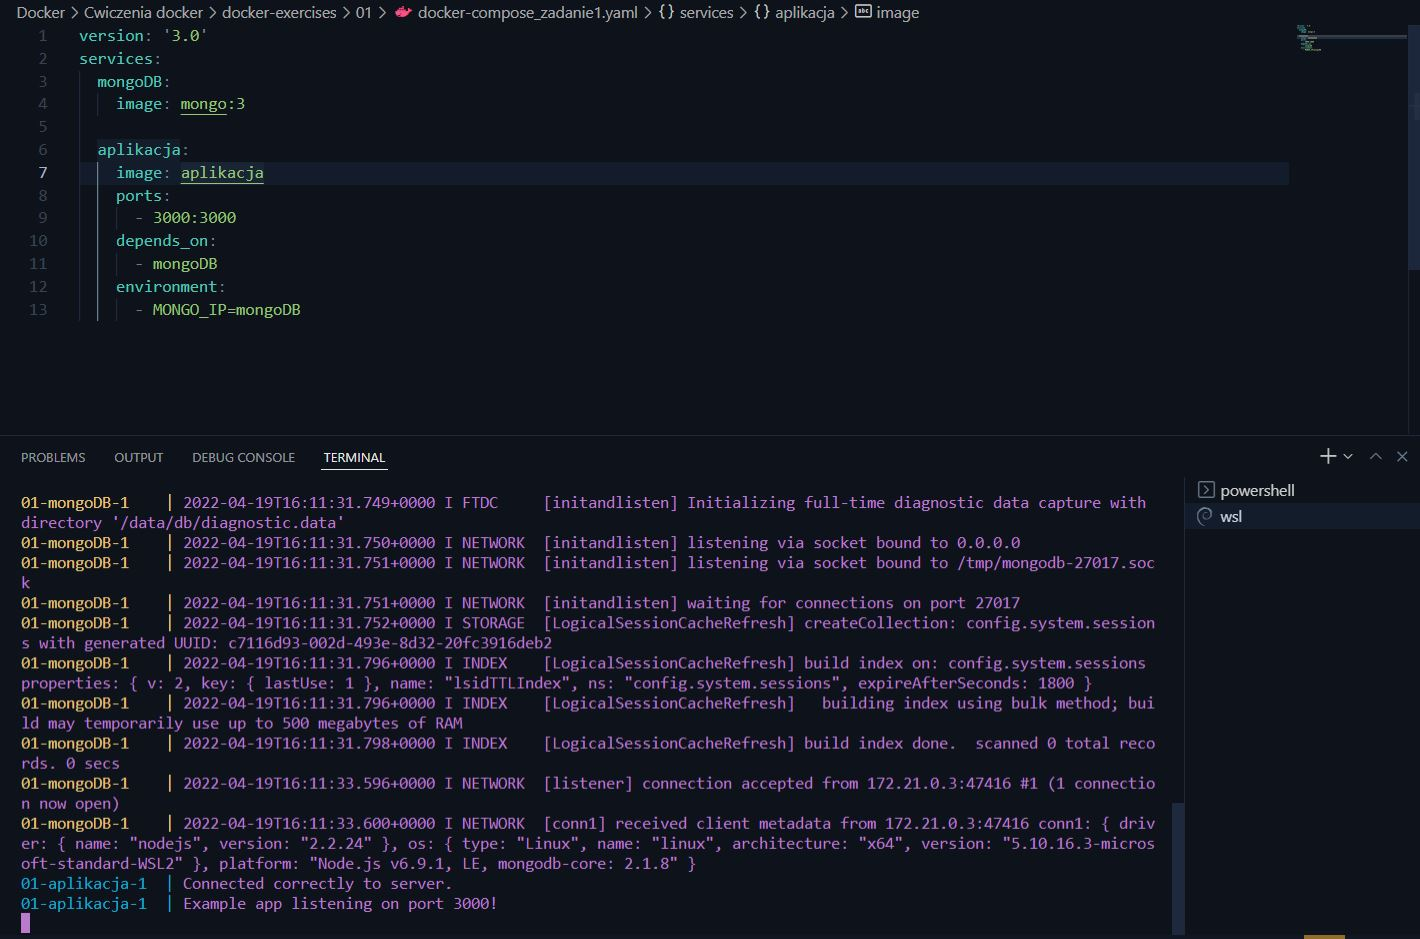
\includegraphics[width=\textwidth]{docker-compose.JPG}
            \caption{Zawartość pliku docker compose oraz wynik egzekucji}
            \label{fig:dockercompose}
        \end{figure}
        Jak widać na powyższym rysunku udało się uruchomić obie usługi, o czym świadczy komunikat \textbf{Connected correctly to server}.
    \subsection{Wynik polecenia curl.}
        \begin{figure}[!h]
            \centering
            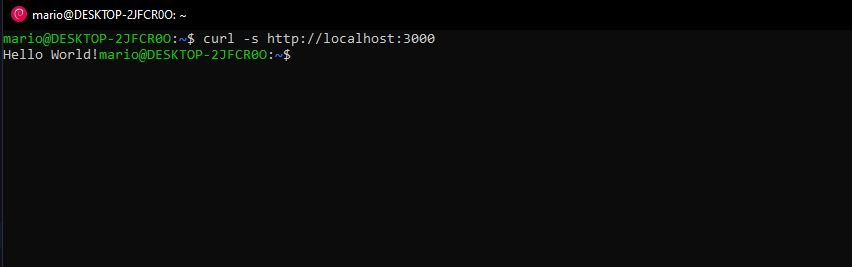
\includegraphics[width=\textwidth]{curl.JPG}
            \caption{Wynik polecenia curl}
            \label{fig:curl}
        \end{figure}
        Jak widać wszystko zostało skonfigurowane poprawnie, ponieważ polecenie curl zwróciło napis \textbf{Hello World!}
    \section{Źródła}
    Autor aplikacji nodejs: github.com/Vizuri
\end{document}
